% Presentation (content) for talk at GPN3
% TYPOGRAPHY
\documentclass[ngerman,draft, usepdftitle=true]{beamer}

\usepackage{fontspec}
\usepackage[shorthands=off]{babel}
\usepackage{csquotes}
\usepackage{graphicx}
\graphicspath{{./images/}}

% fonts for demonstration in LaTeX
% Computer Modern Roman (default); short: cmr
% \usepackage{droidserif} % Antiqua font; short: fdr
\newfontfamily\fontfamilydroidserif{DroidSerif-Regular.ttf}
% \usepackage[rm]{roboto} % Slab Serif font; short: RobotoSlab-LF
\newfontfamily\fontfamilyrobotoslab{RobotoSlab-Regular.ttf}
% \usepackage[sfdefault]{FiraSans} % Sans Serif font; short: FiraSans-ProportionalLF
\newfontfamily\fontfamilyfirasans{FiraSans-Regular.otf}
% \usepackage{yfonts} % Blackletter fonts (Schwabacher); short: yswab
% or \swabfamily
\newfontfamily\fontfamilyfraktur{UnifrakturMaguntia.ttf}
%\newfontfamily\fontfamilyschwabacher{yswab.afm}
% \usepackage{lmodern} % Latin Modern Roman; short: lmr
\newfontfamily\fontfamilylatinmodern{Latin Modern Roman}

\usepackage{calc}
\usepackage{booktabs}

\newcommand*{\code}[1]{\texttt{#1}}

% note settings
\setbeameroption{show notes}

% themes
\usetheme{Singapore}%Frankfurt, Dresden, Rochester
\usecolortheme{seahorse}

% beamer settings
\setbeamercovered{highly dynamic}

% beamer templates
%\setbeamertemplate{logo}{\includegraphics[width=2cm]{\testimage}}
\setbeamertemplate{background canvas}[vertical shading][bottom=gray!30,top=white]
% \newlength{\topbarheight}\setlength{\topbarheight}{.2cm}
% \newlength{\topbaroffset}\setlength{\topbaroffset}{-1.2cm}
% bites with subtitles!!
% \setbeamertemplate{background}{%[grid][step=0.64\paperwidth,color=gray]
%   \color{gray}\rule[\topbaroffset]{2cm}{\topbarheight}%
%   \color{blue!30}\rule[\topbaroffset]{{\paperwidth}}{\topbarheight}
% }

% newcommands
\newcommand{\Beispieltext}{%
  \fontsize{5pt}{6pt}\selectfont
  \fontfamilylatinmodern
  Dies ist ein Beispieltext zu möglichem Textsatz.
  Dies ist ein Beispieltext zu möglichem Textsatz.
  Und dies ist noch mehr Beispieltext zu möglichem Textsatz.
  Dies ist ein Beispieltext zu möglichem Textsatz.
  Dies ist ein Beispieltext zu möglichem Textsatz.
  Und noch mehr Beispieltext zu möglichem Textsatz.
  Dies ist ein Beispieltext zu möglichem Textsatz.
  Und dies ist noch mehr Beispieltext zu möglichem Textsatz.
  Dies ist ein Beispieltext zu möglichem Textsatz.
  Und noch mehr Beispieltext zu möglichem Textsatz.
  Dies ist ein Beispieltext zu möglichem Textsatz.
  Dies ist ein Beispieltext zu möglichem Textsatz.
}

% titlepage
\title{Typographie – ein Einblick}
\author{Gesina Schwalbe}

\begin{document}

% title and table of contents
\maketitle
\tableofcontents[hideallsubsections]%,pausesections]

%------

\section{Was ist Typographie?}
\frame{\sectionpage}
\subsection{Definition}
\begin{frame}
  \begin{quote}
    Typography is the visual component of the written word. \\
    (\href{http://practicaltypography.com/}{Matthew Butterick})
  \end{quote}
  \begin{quote}<2->
    [Typografie ist die] visuelle Gestaltung eines Druckerzeugnisses,
    eines virtuellen Mediums oder einer dreidimensionalen Oberfläche[.]\\
    (\href{http://www.typolexikon.de/typographie/}{Typolexikon})
  \end{quote}
  \begin{quote}<3->
    Typographie ist visuelle Textgestaltung. (ich)
  \end{quote}
  \note<3>{Überall, wo geschriebenes Wort zu finden ist, ist
    Typographie!}
  \note<3>{In diesem Vortrag: Was kann ich alles beachten + Hinweise}
\end{frame}

\begin{frame}[t]{Teilbereiche}
  \begin{block}{Mikrotypographie}<1|only@1>
    Details einzelner Zeichen und direkte Beziehungen
    \begin{itemize}
    \item Zeichensetzung
    \item Schriftart
    \item Zeichen-/Wortabstände, Kerning, Ligaturen
    \end{itemize}
  \end{block}
  \begin{block}{Makrotypographie}<2|only@2>
    Layout; Verhältnisse aller Elemente zueinander
    \begin{itemize}
    \item Seitenformat
    \item Satzspiegel, Zeilenbreite
    \item Schriftgröße, Zeilenabstand, Absatzkennzeichnung
    \item Textsatz, Trennung
    \item Hervorhebungen
    \item Zusatzelemente
    \end{itemize}
  \end{block}
\end{frame}

%---

\subsection{Einfluss von Typographie}
\frame{\subsectionpage}

\begin{frame}
\begin{quote}
  Mithilfe von Typografie kann der Inhalt, Zweck und die Anmutung eines
  Werkes verdeutlicht werden. \\(Wikipedia)
\end{quote}
\end{frame}

\begin{frame}{Beispiele für den Einfluss von Typographie}
  \begin{description}[Aufmerksamkeit]
  \item[Lesbarkeit] 
    Namenschilder \note{Werbung}, 
    Verkehrsschilder
  \item[Aufmerksamkeit] 
    Sicherheitsanweisungen \note{Flugzeugchecklisten}, 
    Dokumentationen \note{NASA}
  \item[Aussage] 
    Bewerbungen, 
    Projektanträge, 
    Mahnbriefe
\end{description}
\end{frame}

%---

\subsection{Historie}
\begin{frame}
  \subsectionpage
  
  \centering
  Wo kommen Gewohnheiten her?
\end{frame}

\begin{frame}{Ursprüngliche Typographie}
  \begin{block}{Duden}
    \begin{enumerate}
    \item Kunst der Gestaltung von Druck-Erzeugnissen nach
      ästhetischen Gesichtspunkten; \alert{Buchdruckerkunst}
    \item typografische Gestaltung (eines Druck-Erzeugnisses)
    \end{enumerate}
  \end{block}
\end{frame}
\begin{frame}{Historische Entwicklung}
  \begin{description}
    \item[Anfänge] Handschrift (kursiv oder gebrochen)
    \item[15.\,Jh.] Buchdruck
    \item[16.\,Jh.] platzsparende Kursivschriften im Druck
    \item[18.\,Jh] Farbdruck/Lithographie \note{erstmals Bildelemente}
    \item[1816] Sans Serif \note{Grotesk nicht sehr alt!}
    \item[1870er] Schreibmaschine \note{großer Einfluss bis heute}
    \item[1970er] Markup Sprachen (GenCode, GML; SMGL als erste standardisiert)
    \item[1984] WYSIWYG (Apple mit MacWrite)
    \item[90er] Internet
  \end{description}
\end{frame}


% ------

\begin{frame}{allgemeine Hinweise}
  \begin{itemize}
  \item<1-> Nutze Formatvorlagen (Word/LibreOffice) oder Markup (HTML,
    LaTeX) für Konsistenz und Wartung.
  \item<2-> Erst das Ziel, dann der Inhalt, zum Schluss der Satz
  \end{itemize}
  \note<2>{Votragsaufbau: vom Detail zum Gesamtbild}
\end{frame}

\section{Mikrotypographie}
\frame{
  \sectionpage
  
  \centering Details der Zeichen
}

\subsection{Zeichenwahl}
\begin{frame}{Die richtigen Zeichen}
  \begin{tabular}{llll}
    \toprule
     & Zeichen & Eingabe & so nicht \\\midrule[\heavyrulewidth]
    Ellipsen & … &\code{AltGr + .} 
                         & ...\\\midrule
    Minus, Gedankenstrich, bis & – & \code{AltGr + -} 
                         & - oder ---\\\midrule
    Anführungszeichen & „“ & \code{AltGr + v/b} 
                         & " oder '\\\midrule
    kleine Wortabstände & z.\,B. & \code{\&thinsp;}, \code{\textbackslash,}
                         &\\\bottomrule
  \end{tabular}
\end{frame}

\begin{frame}{Die richtigen Umbrüche}
  \begin{tabular}{lll}
    \toprule
    & Eingabe & so nicht\\\midrule[\heavyrulewidth]
    Zeilenumbruch & \code{Shift+Enter}, \code{<br/>}
              & kein Absatzumbruch\\\midrule
    Absatzumbruch (¶)& \code{Enter} 
              & keine Leerzeile(n)\\\midrule
    Seitenumbruch &
              & keine 1000 Leerzeilen\\\midrule
    geschütztes Leerz. & \code{Strg+Shift+Leer}%, \code{\&nbsp;}
              & „1. Sep.“ trennen \\\midrule
    weiches Trennz. & \code{Strg + -}, \code{\&shy;}
              & \\\bottomrule
  \end{tabular}
\end{frame}

% ---

\subsection{Schriftarten}
\frame{
  \subsectionpage

  CSS: \code{font-family: <schriftart>;}
}

\begin{frame}{Schriftfamilien}
  \begin{description}[Schriftfamilie]
  \item[Schriftart] ein Zeichensatz in best. Schnitt 
    (z.\,B. Latin Modern Roman Slanted)
  \item[Schriftfamilie] Sammlung zusammengehöriger Schriftarten
    (kursiv, grotesk, monotype, untersch. Schnitte, Kapitälchen)
  \end{description}
\end{frame}

\begin{frame}{Schriftgattungen}
  \begin{block}{Antiqua}
    rundbogige lateinische Schriften
  \end{block}
  \begin{block}{Gebrochene Schriften}
    mittelalterliche Frakturschriften, z.\,B.\\
    {\fontfamilyfraktur Dieser Text ist geschrieben in Unifraktur Matuntia.}
    %{\swabfamily Schwabacher Schriften}
  \end{block}
  \begin{block}{Nichtrömisch}
    Griechisch, Kyrillisch, Arabisch, Chinesisch …
  \end{block}
\end{frame}

\begin{frame}{Untergruppen der Antiqua}
  \begin{block}{Antiqua}<1->
    dreieckige Serifen\\
    \uncover<2->{
      {\fontfamilydroidserif Dieser Text ist geschrieben in Droid
        Serif.}\\
      {\fontfamilylatinmodern Dieser Text ist geschrieben in Latin
        Modern.}
    }
  \end{block}
  \begin{block}{Egyptienne}<3->
    auch \emph{serifenbetonte Linear-Antiqua}; 
    betonte Serifen, glm. Dicke\\
    \uncover<4->{\fontfamilyrobotoslab Dieser Text ist geschrieben in Roboto Slab.}
  \end{block}
  \begin{block}{Grotesk (Sans Serif)}<5->
    serifenlos\\ 
    \uncover<6->{\fontfamilyfirasans Dieser Text ist geschrieben in Fira Sans.}
  \end{block}
\end{frame}

\begin{frame}{Worauf kann man achten?}
  Einige Eigenschaften (immer zuerst Textkörper)
  \begin{block}{Schriftgruppe}<1->
    mit/ohne Serifen (kein Monotype außer für Code)
    \begin{itemize}
    \item Viel Text: Serifen unterstützen Zeilenorientierung
    \item Schlechte Auflösung: Serifenlos wird meist besser
      dargestellt
      \note<1>{Deshalb sind Serifen im Netz so häufig; früher war die
        Bildschirmqualität i.\,A. schlecht.}
    \end{itemize}
  \end{block}
  \begin{block}{Grauwert}<2->
    Flächendeckung der Schrift; betrachte versch. Schnitte\\
    Screen mehr, Druck weniger
  \end{block}
  \begin{block}{Qualität}<3->
    Detailreichtum der Schrift
  \end{block}
\end{frame}

\begin{frame}{Worauf kann man achten?}  
  \begin{block}{Features}<1->
    OpenType Features bei OTF
    (Kapitälchen, Ligaturen, Kerning, Alternative Zahlen …)
  \end{block}
  \begin{block}{Weite}<2->
    Wie dicht ist die Schrift?
    \note<2>{Beispiel einer dichten Schrift: Times New Roman (Zeitung)}
  \end{block}
  \begin{block}{Wirkung}<3->
    Modern/gediegen? Seriös/lustig?
  \end{block}
  \begin{block}{Kosten}<4->\end{block}
\end{frame}

\begin{frame}{Schriften vergleichen}
  gleichen Text auf selbe Höhe bringen, vergleichen
  
  \alert{Nicht Comic Sans}

  %% INSERT Schriftenvergleich
\end{frame}

\begin{frame}{Mischen von Schriften}
  \begin{alertblock}{Nicht zu viele versch. Schriftfamilien}<1->
    Stiftet Verwirrung und Schriftdateien werden eingebettet
  \end{alertblock}
  \begin{alertblock}{Auf Konsistenz achten}<2->
    Erst die Hauptschriftart und die anderen daran orientiert
  \end{alertblock}
\end{frame}

%---

\subsection{Beziehungen zwischen Zeichen}
\begin{frame}{Ligaturen}
Buchstabenverbund für schönere Abstände/Überlappungen
\begin{center}
  
\includegraphics[height=.2\paperheight]{Ligatures.png}
\end{center}
\vfill
CSS: \code{text-rendering: optimizeLegibility;}
\end{frame}

\begin{frame}{Kerning}
Anpassen des Zeichenab-/überstands bei best. Zeichenpaaren
\begin{center}
  
\includegraphics[height=.2\paperheight]{Kerning_without.png}
  \hfill
  
\includegraphics[height=.2\paperheight]{Kerning_with.png}
\end{center}
\vfill
CSS:\\ 
\code{text-rendering: optimizeLegibility; \\
  <browser-prefix>font-feature-settings: kern;}
\end{frame}

%------

\section{Makrotypographie}
\begin{frame}
  \sectionpage

  \centering
  Das Gesamtbild
  \note{Von wichtigen Teilen (Textkörper) zu unwichtigen (Metadaten, Hervorhebungen)
    Von Essentiellem zu Ästhetik}
\end{frame}

\subsection{Layout}
\begin{frame}
  \subsectionpage
  \centering
  essentielle Überlegungen: \\
  ersten Eindruck festlegen 
  mit \emph{Grauwert} und \emph{Grobstruktur}
\end{frame}

\begin{frame}{Schrift-/Hintergrundfarbe}
  \begin{block}{Druck}<1->
    \begin{itemize}
    \item Möglichst hoher Kontrast
    \item Schwarz auf Weiß (Kosten)
      \note<1>{Keine zu sehr ablenkenden Farben}
    \end{itemize}
  \end{block}
  \begin{block}{Screen, Beamer}<2->
    \begin{itemize}
    \item Kontrast verringern (Bildschirme leuchten aktiv)
    \item Keine irritierenden/beißenden Farben
    \end{itemize}
  \end{block}
\end{frame}

\begin{frame}{Schriftgröße}
  \begin{description}[Screen (insb. Web)]
  \item[Druck] 10–12pt (kurze Lesedistanz)
  \item[Screen (insb. Web)] 15–20px
  \item[Präsentation] nicht zu klein
  \end{description}
  \vfill
  CSS: \code{font-size: …px}
\end{frame}

\begin{frame}{Zeilenabstände}
  Faustregel: 120–140\% der Schriftgröße
  \begin{columns}[onlytextwidth,T]
    \begin{column}{.3\paperwidth}
      \fontsize{8pt}{8.8pt}\selectfont
      \fontfamilylatinmodern
      110\%:
      Dies ist ein Beispiel für Abstände zwischen Zeilen.
      Dies ist ein Beispiel für Abstände zwischen Zeilen.
      Dies ist ein Beispiel für Abstände zwischen Zeilen.
    \end{column}
    \begin{column}{.3\paperwidth}
      \fontsize{8pt}{10.4pt}\selectfont      
      \fontfamilylatinmodern
      130\%:
      Dies ist ein Beispiel für Abstände zwischen Zeilen.
      Dies ist ein Beispiel für Abstände zwischen Zeilen.
      Dies ist ein Beispiel für Abstände zwischen Zeilen.
    \end{column}
    \begin{column}{.3\paperwidth}    
      \fontsize{8pt}{13.6pt}\selectfont
      \fontfamilylatinmodern
      170\%:
      Dies ist ein Beispiel für Abstände zwischen Zeilen.
      Dies ist ein Beispiel für Abstände zwischen Zeilen.
    \end{column}
  \end{columns}
  \vfill
  CSS: \code{line-heigt: 1.3} (ohne Einheit)
\end{frame}

\begin{frame}{Absatzabstände}
  \begin{itemize}
  \item<1-> Abstand \alert{oder} Einzug (\alert{keine} Leerzeile)
    \begin{description}
    \item[Abstand] 50–100\% der Schriftgröße\\
      CSS: \code{p \{margin-bottom: 0.75;\}}
    \item[Einzug] 1–4em (1em $\approx$ Schrifthöhe)\\
      CSS: \code{p \{text-indent: …em;\}} \note{em wird in px umgerechnet}
    \end{description}
  \item<2-> Schusterjungen und Hurenkinder verhindern
  \end{itemize}
\end{frame}

\begin{frame}{Satzspiegel}
  \begin{itemize}
  \item max. Zeilenbreite 2–3 Alphabete 
    \note{sonst geht Zeilenbezug verloren}
  \item evtl. mehrere Spalten (nicht zu viele!)
  \item genügend Rand (Grauwert)
  \item Textbereich sinnvoll platzieren\\
    (einseitig: zentriert, doppelseitig: innen)
  \end{itemize}
\end{frame}

\begin{frame}{Beispiel Satzspiegelkonstruktion}
  Für begrenzte Textfläche z.\,B.
  \begin{block}{Rasterteilung}
    \centering
    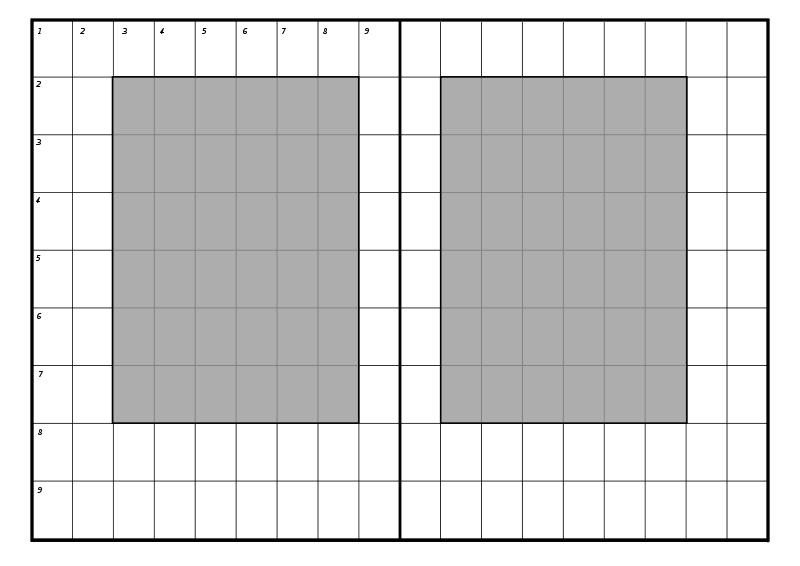
\includegraphics[height=.6\textheight]{Satzspiegel-Rasterteilung.png}
  \end{block}
  Bindekorrektur nicht vergessen!
\end{frame}

\subsection{Textsatz}
\begin{frame}{Textsatz}
  Zu vermeiden
  \begin{itemize}
  \item (ungleichmäßiger) Flatterrand
  \item zu großer (autom.) Wortabstand
  \end{itemize}
  \begin{columns}[T]
    \begin{column}{.3\paperwidth}
      \parbox[t]{\textwidth}{\raggedright\Beispieltext}
    \end{column}
    \begin{column}{.3\paperwidth}
      \parbox[t]{\textwidth}{\Beispieltext}
    \end{column}
    \begin{column}{.3\paperwidth}
      \parbox[t]{\textwidth}{\centering\Beispieltext}
    \end{column}
  \end{columns}
\end{frame}

\begin{frame}{Textsatz – Empfehlungen}
  \begin{description}[schmal/keine Trennung mögl.]
  \item[breit]  Worttrennung einschalten, Blocksatz
  \item[schmal/keine Trennung mögl.] Linksbündig
  \item[nur kurze Passagen] Zentriert
  \item[mögl. nie im Textkörper] Rechtsbündig (Orientierung geht verloren)
  \end{description}
\end{frame}

\begin{frame}{Worttrennung}
  Benutzen!
  \begin{itemize}
  \item<1-> \emph{optionale Umbruchstellen}\\
    LibreOffice: \code{Strg + -}, HTML: \code{\&shy;}
  \item<2-> \emph{geschützte Leerzeichen}(/Bindestriche), insb. bei
    E-Mail-/Webadressen\\
    LibreOffice: \code{Strg+Shift+Leer}, HTML: \code{\&nbsp;}
  \item<3-> Überschriften etc.: \emph{Zeilenumbruch} manuell einfügen \\
    LibreOffice: \code{Shift + Enter}, HTML: \code{<br/>}
  \end{itemize}
  \vfill
  CSS: \code{hyphens: auto;} (magere Unterstützung)
\end{frame}

\subsection{Hervorhebungen}
\begin{frame}
  \subsectionpage
  \centering
  Weniger ist mehr, überdecke den Inhalt nicht
\end{frame}

\begin{frame}{So nicht hervorheben}
  \alert{Generell:} Möglichst wenig hervorheben
  \begin{alertblock}{Nicht unterstreichen!}
    \begin{itemize}
    \item Schreibmaschinen-Gewohnheit
    \item \underline{Unterstreichen ist mit billig} konnotiert
    \end{itemize}
  \end{alertblock}
  \begin{alertblock}{Nicht zu viele Farben!}
    \fontsize{14pt}{18pt}\selectfont
    \frame{\fcolorbox{cyan}{black}{\color{red}Zu \color{green}viele
      \color{yellow}kontrastierende
      \color{blue}Farben
      \color{pink}lenken
      \color{magenta}ab!
    }}
  \end{alertblock}
\end{frame}

\begin{frame}[t]{Hervorheben im Fließtext}  
  % Möglichkeiten im Fließtext: Kursiv, Fett, Kapitälchen, Farbe, 
  % NICHT Unterstreichen/Versalien (aus Schreibmaschinenzeiten)
  % Bei allen: Nur kurze Passagen, keine Absätze (Lesbarkeit)
  \begin{block}{\itshape Kursiv}<1->
    \begin{itemize}
    \item im \textit{Fließtext} zu bevorzugen
    \item bei \textit{Grotesk} meist zu schwach
    \end{itemize}
  \end{block}
  \begin{block}{\bfseries Fett}<2->
    \begin{itemize}
    \item sehr \textbf{auffällig} durch Kontrast
    \item \textbf{Abstufungen} beachten!
    \end{itemize}
  \end{block}
  \begin{block}{\scshape Kapitälchen}<3->
    \begin{itemize}
    \item etwa wie fett, meist \textsc{schwerer lesbar}
    \item nur gute verwenden: \textsc{Grauwert} oft zu schwach
    \end{itemize}
  \end{block}
\end{frame}

\begin{frame}[t]{Hervorheben im Fließtext}
  \begin{block}{\uppercase{Versalien}}<1->
    \begin{itemize}
    \item \uppercase{sehr} auffällig, \uppercase{schwer lesbar}
    \item auf \uppercase{Zeichenabstand} achten, nicht mit Capslock
    \end{itemize}
  \end{block}
  \begin{block}{Farbe}<2->
    \begin{itemize}
    \item {\color{green}Kontrast} hängt vom Grauwert ab – ausprobieren
    \item auf {\color{green}Konsistenz} achten (nicht zu viele kontrastierende)
    \item Druckkosten
    \end{itemize}
  \end{block}  
\end{frame}

\begin{frame}{Hervorheben im Fließtext}
  \begin{alertblock}{Beachte:}
    Oft sind \emph{Emphasize}-Umgebungen/-Vorlagen
    gegeben\\
    \begin{description}
    \item[LibreOffice] Character-Styles
    \item[HTML] \code{<emph>}
    \item[\LaTeX] \code{\textbackslash emph}
    \end{description}
  \end{alertblock}
\end{frame}

\begin{frame}{Sonstiges Hervorheben}
\begin{block}{Weißraum (vertikaler Abstand)}<1->
  \emph{Reden ist Silber, Schweigen ist Gold.}
\end{block}
\begin{block}{Einrücken (horizontaler Abstand)}<2->
  nicht zu viel (Zeilenorientierung)
  \note<2>{NICHT zentrieren (zu große Einrückung -> Bezug zum Text geht verloren)}
\end{block}
\begin{block}{Schriftgröße}<3->
  kleinstmögliche erkennbare Schritte machen
  \note<2>{schlechtes Beispiel: HTML-Default der Überschriften}
\end{block}
\begin{block}{Rahmen (z.\,B. Code-Blocks)}<4->
  \begin{itemize}
  \item nicht zu auffällig in Dicke/Effekt (überdeckt umrahmtes!)
  \item nicht zu dünn (digital nicht darstellbar)
  \end{itemize}
  \fbox{CSS: \code{border}}
\end{block}
\end{frame}

\begin{frame}{Hervorheben}
\centering
\emph{Grundsätzlich:~}

\vspace*{1.5\baselineskip}
Weniger ist mehr\\ – \\
kleinstmögliche Hervorhebung für den gewünschten Effekt nutzen
\end{frame}


\subsection{Sonderelemente}
\begin{frame}
  \subsectionpage
  \centering
  Alles außer Fließtext – ein paar Beispiele
\end{frame}

\begin{frame}{Tabellen}
  \begin{block}{Rahmen}<1->
    nicht zu auffällig; Steigerung:
    \begin{enumerate}
    \item nur Trennlinien (oben, unten)
    \item horizontale
    \item vertikale
    \end{enumerate}
    CSS: \code{border-width}, \code{border}
  \end{block}
  \begin{block}{Abstände}
    CSS: \code{padding}
  \end{block}
\end{frame}

\begin{frame}{Tabellen – Beispiel}
  \begin{description}
  \item[zu viel]~
    \parbox[t]{.5\textwidth}{
      \fontsize{8pt}{10.4pt}\selectfont
      \begin{tabular}{|l|c|l|}
        \hline
        Bezeichnung & Zeichen & UTF-8\\\hline
        Hyphen Minus & - & \code{U+002D}\\\hline
        En Dash & – & \code{U+2013}\\\hline
        Em Dash & --- & \code{U+2014}\\\hline
      \end{tabular}
      \\[\baselineskip]\mbox{}}

  \item[reicht völlig]~
    \parbox[t]{.5\textwidth}{
      \fontsize{8pt}{10.4pt}\selectfont
      \begin{tabular}{lcl}
        \toprule
        Bezeichnung & Zeichen & UTF-8\\\midrule[\heavyrulewidth]
        Hyphen Minus & - & \code{U+002D}\\
        En Dash & – & \code{U+2013}\\
        Em Dash & --- & \code{U+2014}\\\bottomrule
      \end{tabular}
      \\[\baselineskip]\mbox{}}

  \item[in Ordnung]~
    \parbox[t]{.5\textwidth}{
      \fontsize{8pt}{10.4pt}\selectfont
      \begin{tabular}{lcl}
        \toprule
        Bezeichnung & Zeichen & UTF-8\\\midrule[\heavyrulewidth]
        Hyphen Minus & - & \code{U+002D}\\\midrule
        En Dash & – & \code{U+2013}\\\midrule
        Em Dash & --- & \code{U+2014}\\\bottomrule
      \end{tabular}
      \\[\baselineskip]\mbox{}}
  \end{description}
\end{frame}

\begin{frame}{Formeln}
  \begin{block}{Fließtextformeln}
    Nicht zu lang – lieber zu viel als zu wenig absetzen
  \end{block}
  
  \begin{beamerboxesrounded}[shadow=true]{Beispiel}
    \fontsize{9pt}{12pt}\selectfont\fontfamilylatinmodern
    Die Formel $E=m\cdot c^2$ ist für Fließtext noch gut geeignet.
    Das etwas längere $\tau_{-\gamma(\O)}\colon E_2\to E_2$ auch noch,
    aber 
    $\Omega(T+S)(f)
    = \tau^*_{T+S}(f)
    = f\circ\tau_{T+S} 
    = f\circ\tau_{S+T}
    = f\circ\tau_{S}\circ\tau_{T}
    = \tau^*_T\circ\tau^*_S(f)
    = \Omega(T)\circ\Omega(S)(f)$
    sollte definitiv abgehoben werden, in \LaTeX z.\,B. mit der
    \code{align}-Umgebung
    \begin{align*}
      \Omega(T+S)(f)
      &= \tau^*_{T+S}(f)\\
      &= f\circ\tau_{T+S} 
        = f\circ\tau_{S+T}
        = f\circ\tau_{S}\circ\tau_{T}\\
      &= \tau^*_T\circ\tau^*_S(f)
        = \Omega(T)\circ\Omega(S)(f)
    \end{align*}~\\
  \end{beamerboxesrounded}
\end{frame}

\begin{frame}{Bilder}
  Textfluss nicht zerreißen – lieber referenzieren
%% INSERT EXAMPLE
\end{frame}

%------

\section{Beispiele}

%------

\begin{frame}{Wo kann ich noch mehr lernen?}{(auch genannt: Quellen)}
\begin{itemize}
  \item Wikipedia
  \item \url{http://practicaltypography.com/} von Matthew Butterick
  \item \url{http://www.typolexikon.de/}: alles über Typographie
  \item \textbf{Type:Rider} (\url{https://bulkypix.com/games/typerider/})
  \item \url{http://www.identifont.com/}: Schriften surfen
  \end{itemize}
\end{frame}


  % ====================

% \subsection{<first section:first subsection>} 
% \frame{
%   \frametitle{<frame of first subsection>}
%   \framesubtitle{<some subtitle for this frame>}
%   And the first subsection.
% }
% \section{<second section>}
% \frame{Text underneath second section.}
% \frame{\tableofcontents[hideothersubsections]}

% % frame options, againframe
% \subsection{frame options}
% \frame[plain,squeeze,label={plainframe}]{
%   \frametitle{<this is a plain frame>}
%   And a little within the first subsection.
  
%   One can only see the manually set shading of the background canvas
%   and the two colored rules of the background.

%   By the way: This is squeezed.

%   Oh and this frame should appear twice because of againframe.
% }
% \againframe[plain]{plainframe}

% \subsection{<second section:second subsection>}
% \frame{Text of second subsection.}
% \section{<third section>}
% \frame{
%   \frametitle{<frametitle directly underneath third section>}
%   Text of third section.
% }

% \part{<Second Part>}
% \frame{\partpage}
% \frame{\tableofcontents}


% % multicolumn
% \section{multicolumn}
% \begin{frame}
%   \frametitle{Some experiments with columns}
%   \begin{columns}[onlytextwidth,T]
%     \begin{column}{.3\textwidth} 
%       really extremely many not to say
%       an uncountable amount of blubbles
%     \end{column}
%     \begin{column}{.2\textwidth} 
%        a little less blubbles, since this
%      one is thinner …
%      \end{column}
%      \begin{column}{.1\textwidth}
%        extremely thin column without blubbles
%      \end{column}
%   \end{columns}
% \end{frame}

% % layers
% \section{layers}
% \frame{\tableofcontents[currentsection]}
% \begin{frame}
%   \textbf<1|alert@2>{Here} you have 
%   \pause an \alt<1-7>{enumeration (from 1-7)}{iteration afterwards}:
%   \alt<1-7>{%
%   \begin{enumerate}
%     \item<2-4> 2-3
%     \item<2-4|invisible@3> also 2-3 but invisible at 3 
%     \item<+-> from 2 to end
%     \item<4-> from 4 onwards \only<5>{(some only text)} and some text
%     \item<+-> from 3 to end \uncover<6>{(some uncovered text)} and some text
%     \item<+-> from 4 to end \visible<7>{(some visible text)} and some text
%   \end{enumerate}
%   }{%
%     \begin{iterate}
%       \item<1-2> This should never be visible.
%       \item<+-> This should be visible now to the end, in contrast
%         to the one before.
%     \end{iterate}
%   }
%   And some changing fruit: \temporal<3-5>{appel}{orange}{banana}
% \end{frame}


% \section{boxes}
% \subsection{simple boxes}
% \begin{frame}{several simple blocks}
%   \begin{block}{a simple block}
%     Text within a simple block.
%   \end{block}
%   \begin{alertblock}{alert block}
%     Some important text within an alert box!
%   \end{alertblock}
%   \begin{exampleblock}{example block}
%     This could be an example.
%   \end{exampleblock}
% \end{frame}

% \subsection{fancy boxes}
% \begin{frame}{fancy boxes}
%   \begin{beamerboxesrounded}[width=.5\textwidth,shadow=true]{beamerbox}
%     This is a rounded beamer box. With shadow.
%   \end{beamerboxesrounded}
%   \setbeamercolor{some color}{fg=green, bg=black,}
%   \begin{beamercolorbox}[wd=.7\textwidth,ht=2cm,dp=2cm,%
%     shadow=true,rounded=true,center]%
%     {some color}
%     This is a beamercolorbox with
%     \begin{description}
%       \item[\texttt{fg=green}] green text
%       \item[\texttt{bg=black}] black background
%     \end{description}
%   \end{beamercolorbox}
% \end{frame}

% \section{picture handling}
% \begin{frame}[fragile]{pictures}
% \begin{verbatim}
% \includegraphics<+->[width=1cm]{\testimage}
% \end{verbatim}
%   \includegraphics<+->[width=1cm]{\testimage}

% \begin{verbatim}
% \pgfdeclareimage[width=2cm]{mylogo}{./\testimage}
% \pgfuseimage<2->{mylogo}
% \end{verbatim}
% \pgfdeclareimage[width=2cm]{mylogo}{./\testimage}
% \pgfuseimage<2->{mylogo}
% \end{frame}

% % frames with lots of text …
% \frame[allowframebreaks=0.5]{
%   \blindtext
%   \note{This is some note}
%   \blindtext
% }


\end{document}
